% vim: set foldmethod=marker foldlevel=0:

\documentclass[a4paper]{article}
\usepackage[UKenglish]{babel}

\usepackage{preamble}

\usepackage{graphicx}
\graphicspath{ {./imgs/} }

\fancyhead[L]{MA146 Assignment 1}
\title{MA146 Methods of Mathematical Modelling 1, Assignment 1}
\colorlet{questionbodycolor}{green!50!teal!50}

\begin{document}

\maketitle

\setlength{\parindent}{0em}
\setlength{\parskip}{1em}

% {{{ Q1
\question{1}

\begin{questionbody}
For the following models, classify the system (discrete or continuous, deterministic or
stochastic) and the questions (forward, inverse, or control problem)
\end{questionbody}

\subsection{~} % 1.a

\begin{questionbody}
Suppose that the amount $u(t)$ of a drug in the blood stream satisfies a differential equation of the form \[
\diff t u(t) = s(t) - r u(t).
\]
Here, $s(t) \ge 0$ is the supply and $r > 0$ is a factor related to the degradation of the drug.

From some blood samples taken at different times, therapists measure the drug amount and then want to determine $r$.
\end{questionbody}

This is a continuous, deterministic system and an inverse problem.

\subsection{~} % 1.b

\begin{questionbody}
An internet server receives requests at random times and stores them in a queue. They are processed at a rate that depends on the number of requests in the queue (by allocating more computing nodes when the number is high).

The managers want to allocate computing power such that all requests are processed within a certain time of arrival with a probability above 95\%.
\end{questionbody}

This is a discrete, stochastic system and a control problem.

\newpage
\subsection{~} % 1.c

\begin{questionbody}
We consider how a piece of information spreads in a social network. By $i_k$ we denoted the number of participants that are reached at a time $t_k = k \Delta t$ where $\Delta t > 0$ is a given time interval. We believe that \[
i_k = i_{k-1} + r i_{k-1} (b - i_{k-1})
\]
Here, $r \in \N$ is a growth factor and $b$ represents the maximal number of participants, both of which are known.

We'd like to know how many participants are in the know after one hour, half a day, and two weeks.
\end{questionbody}

This is a discrete, stochastic system and a forward problem.

% }}}

% {{{ Q2
\newquestion{2}

\begin{questionbody}
In this question we stuy linear second order equations with constant coefficients of the form \begin{equation}
a \ddd{2}{}{t} x(t) + b \diff x(t) + c x(t) = 0, \quad t \in \R
\label{eqn:general-second-order}
\end{equation}
where $a, b, c \in \R$ are given numbers and $a \ne 0$. One way to find solutions of \eqref{eqn:general-second-order} is by substituting $x(t) = \e^{\lambda t}$ for some $\lambda \in \C$ into the equation. This yields $a \lambda^2 \e^{\lambda t} + b \lambda \e^{\lambda t} + c e^{\lambda t} = 0$.

After dividing by $\e^{\lambda t} \ne 0$ we obtain the \textit{auxiliary equation} \[
a \lambda^2 + b \lambda + c = 0.
\]

Its solutions are given by \[
\lambda_{1,2} = -\f b{2a} \pm \f 1{2a} \sqrt{b^2 - 4ac}.
\]

If $b^2 - 4ac > 0$ then the solutions $\lambda_1 \ne \lambda_2$ are real. Two solutions to \eqref{eqn:general-second-order} then are given by $x_1(t) = \e^{\lambda_1 t}$ and $x_2(t) = \e^{\lambda_2 t}$.

The \textit{complementary function} (or \textit{general solution}) \[
x(t) = l_1 x_1(t) + l_2 x_2(t) = l_1 \e^{\lambda_1 t} + l_2 \e^{\lambda_2 r}, \quad l_1, l_2 \in \R
\] describes all solutions to \eqref{eqn:general-second-order}.

If $b^2 - 4ac < 0$ then we write $\lambda_1 = -\f b{2a} + \mathbf{i} \omega \in \C$ with $\omega = \f 1{2a} \sqrt{4ac - b^2} \in \R$ and note that $\lambda_2 = -\f b{2a} - \mathbf{i} \omega = \overline{\lambda_1}$.
Two real-values solutions of \eqref{eqn:general-second-order} then are $x_1(t) = \e^{-\f b{2a} t} \cos(\omega t)$ and $x_2(t) = \e^{-\f b{2a} t} \sin(\omega t)$, and the \textit{complementary function} is given by \[
x(t) = l_1 x_1(t) + l_2 x_2(t) = l_1 \e^{-\f b{2a} t} \cos(\omega t) + l_2 \e^{-\f b{2a} t} \sin(\omega t), \quad l_1, l_2 \in \R
\]
\end{questionbody}

\newpage
\subsection{~} % 2.a

\begin{questionbody}
In the case $b^2 - 4ac < 0$ with complex solutions of the auxiliary equation, show that $x_2(t)$ is indeed a solution of \eqref{eqn:general-second-order}.
\end{questionbody}

We have $x_2(t) = \e^{-\f b{2a} t} \sin(\omega t)$ and derivatives \begin{align*}
x_2'(t) &= \e^{-\f b{2a} t} \omega \cos(\omega t) - \f b{2a} \e^{-\f b{2a} t} \sin(\omega t) \\
&= \e^{-\f b{2a} t} \l( \omega \cos(\omega t) - \f b{2a} \sin(\omega t) \r)
\end{align*}
\begin{align*}
x_2''(t) &= \e^{-\f b{2a} t} \l(
-\omega^2 - \f{b\omega}{2a} \cos(\omega t)
-\f b{2a} \l( \omega \cos(\omega t) - \f b{2a} \sin(\omega t) \r)
\r) \\
&= \e^{-\f b{2a} t} \l(
\l( \f{b^2}{4a^2} - \omega^2 \r) \sin(\omega t) - \f{b\omega}a \cos(\omega t)
\r)
\end{align*}

We plug these into \eqref{eqn:general-second-order} and get \begin{align*}
&\quad \e^{-\f b{2a} t} \Bigg( a \l( \l( \f{b^2}{4a^2} - \omega^2 \r) \sin(\omega t) - \f{b\omega}a \cos(\omega t) \r) \\
& \qquad + b \l( \omega \cos(\omega t) - \f b{2a} \sin(\omega t) \r) + c \sin(\omega t) \Bigg) \\
%
&= \e^{-\f b{2a} t} \l( \f{b^2}{4a} - a\omega^2 - \f{b^2}{2a} + c \r) \sin(\omega t) \\
&= \e^{-\f b{2a} t} \l( -\f{b^2}{4a} - a\omega^2 + c \r) \sin(\omega t)
\end{align*}

Recall that $\omega = \f1{2a} \sqrt{4ac - b^2}$ so $\omega^2 = \f1{4a^2} (4ac - b^2)$. Therefore \eqref{eqn:general-second-order} becomes \begin{align*}
&\quad \e^{-\f b{2a} t} \l( -\f{b^2}{4a} - \f{4ac}{4a} + \f{b^2}{4a} + c \r) \sin(\omega t) \\
&= \e^{-\f b{2a} t} \times 0 \times \sin(\omega t) \\
&= 0
\end{align*} as expected.

\newpage
\subsection{~} % 2.b

\begin{questionbody}
Find the complementary function of \eqref{eqn:general-second-order} with $a = 2$, $b = -4$, and $c = -6$.
\end{questionbody}
%
\begin{align*}
b^2 - 4ac &= 16 + 8 \times 6 \\
&= 64 \\
\lambda_{1,2} &= \f{4 \pm \sqrt{64}}4 \\
&= 1 \pm 2 \\
x(t) &= l_1 \e^{3t} + l_2 \e^{-t}
\end{align*}

\subsection{~} % 2.c

\begin{questionbody}
Find the complementary function of \eqref{eqn:general-second-order} with $a = -2$, $b = 3$, and $c = -\f54$.
\end{questionbody}
%
\begin{align*}
b^2 - 4ac &= 9 - 5 \times 2 \\
&= -1 \\[1ex]
\lambda_{1,2} &= \f34 \pm \mathbf{i} \f1{-4} \sqrt{1} \\[1ex]
&= \f34 \mp \mathbf{i} \f24 \\[1ex]
x(t) &= \e^{\f34 t} \l( l_1 \cos \f{-t}{4} + l_2 \sin \f{-t}{4} \r)
\end{align*}

\subsection{~} % 2.d

\begin{questionbody}
Find the complementary function solution of \eqref{eqn:general-second-order} with $a = -2$, $b = 0$, and $c = -18$ and then find numbers $l_1, l_2$ such that the solution also satisfies \[
x(2\pi) = 15, \quad \diff t x(2\pi) = 12.
\]
\end{questionbody}
%
\begin{align*}
b^2 - 4ac &= 0 - 8 \times 18 \\
&= -144 \\[1ex]
\lambda_{1,2} &= \f{0 \pm 12 \mathbf{i}}{-4} \\[1ex]
&= \pm 3 \mathbf{i} \\[1ex]
x(t) &= \e^{0t} \l( l_1 \sin 3t + l_2 \cos 3t \r)
\end{align*}

\begin{align*}
x(t) &= l_1 \sin 3t + l_2 \cos 3t \\
x'(t) &= 3 l_1 \cos 3t - 3 l_2 \sin 3t \\
x(2\pi) &= l_1 \sin 6\pi + l_2 \cos 6\pi \\
&= 0 + l_2 \\
l_2 &= 15 \\
x'(2\pi) &= 3 l_1 \cos 6\pi - 3 l_2 \sin 6\pi \\
&= 3 l_1 + 0 \\
3 l_1 &= 12 \\
l_1 &= 4 \\
\thf x(t) &= 4 \sin 3t + 15 \cos 3t
\end{align*}

\subsection{~} % 2.e

\begin{questionbody}
Download the Jupyter notebook \texttt{MA146\_Assignment1.ipynb}. The problem from part \textbf{(d)} is symbolically solved and its solution is displayed.

Run the notebook with the parameters $a = 3$, $b = 12$, $c = 12$ and the initial conditions $x(0) = -4$, $\diff x(0) = 2$.

Submit the code where the initial condition is implemented and the output that displays the solution.

Furthermore, retrieve the solution $x(t)$ from the notebook and show with \enquote{pen and paper} that it indeed satisfies the differential equation \eqref{eqn:general-second-order}.
\end{questionbody}

\begin{figure}[hbtp]
	\centering
	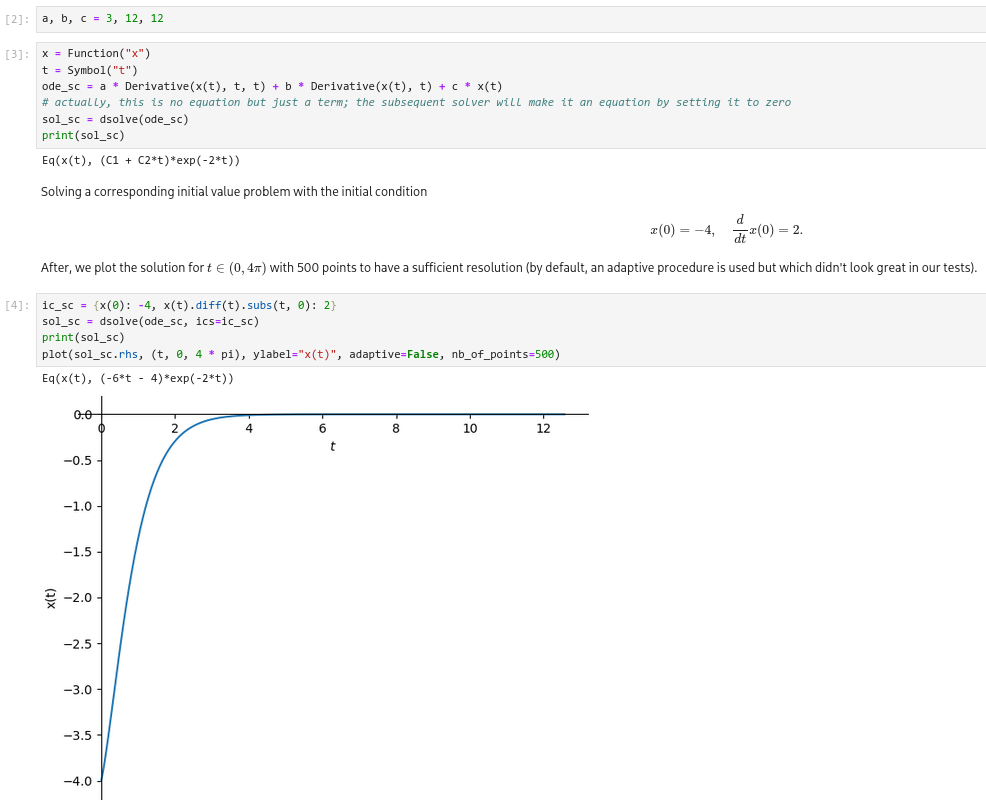
\includegraphics[width=\linewidth]{Q2-e}
	\caption{The code for \textbf{Q2 (e)}}
\end{figure}

The solution given by the notebook is \[
x(t) = (-6t - 4) \e^{-2t}
= -(6t + 4) \e^{-2t}
\]

We differentiate twice and get \begin{align*}
x'(t) &= 2(6t + 4) \e^{-2t} - 6 \e^{-2t} \\
&= (12t + 2) \e^{-2t} \\
x''(t) &= -2(12t + 2) \e^{-2t} + 12 \e^{-2t} \\
&= (-24t + 8) \e^{-2t}
\end{align*}

Plugging this into \eqref{eqn:general-second-order} gives \begin{align*}
& 3 (-24t + 8) \e^{-2t} + 12 (12t + 2) \e^{-2t} - 12 (6t + 4) \e^{-2t} \\
&= \e^{-2t} \l( -72t + 24 + 144t + 24 - 72t - 48 \r) \\
&= \e^{-2t} \times 0 \\
&= 0
\end{align*} as expected.

\subsection{~} % 2.f

\begin{questionbody}
Consider now the parameters $a = 1.0$, $b = −0.2$, and $c = 8.0$. Use the notebook to solve the differential equation three times with initial data $x(0) \in \{1.5, 2.0, 2.7\}$ and always $\diff t x(0) = 0$.

Generate a parametric plot displaying all solutions for $t \in (0, 4\pi)$ in the same graph.
\end{questionbody}

\begin{figure}[hbtp]
	\centering
	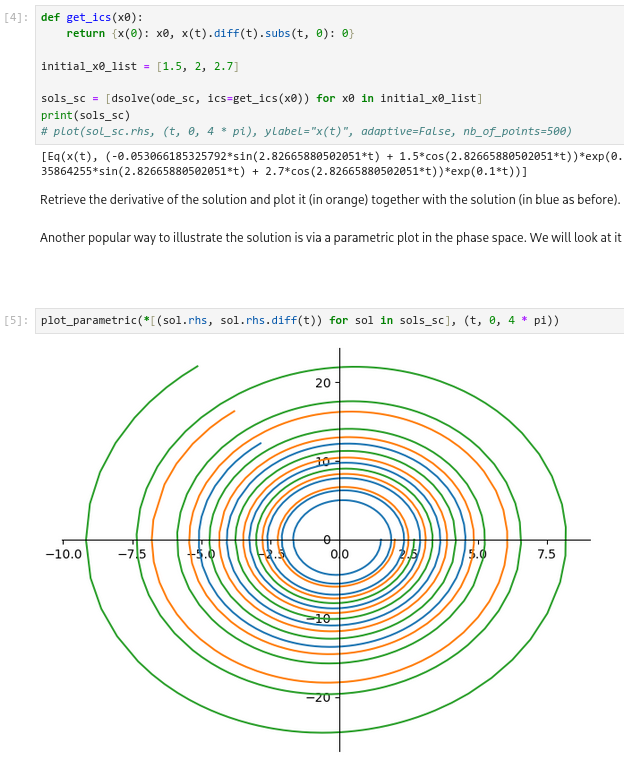
\includegraphics[width=\linewidth]{Q2-f}
	\caption{The code for \textbf{Q2 (f)}}
\end{figure}

% }}}

% {{{ Q3
\newquestion{3}

\begin{questionbody}
Let us work out the height $h(t)$ as a function of time $t$ during a bungee jump.

Assuming that the jumper just drops the initial velocity is zero, $\dot h(0) = 0$, and to have a height reference we also set the initial height to zero, $h(0) = 0$. By Newton’s law \[
m \ddot h(t) = f(t), \quad t > 0
\] where $m > 0$ is the mass of the jumper (assumed a point mass, we don’t account for their shape) and $f$ is the force acting on them. We neglect air resistance and for now assume that the cliff or bridge is high enough so that the jumper could enjoy it a second time (so $h(t)$ is unlimited from below).

Denote the length of the rope with $\ell > 0$. Whilst the jumper is in free fall, gravitation is the only force acting on them, hence \[
f(t) = -mg, \quad \text{when } h(t) \ge -\ell
\] with the gravitation constant $g$. Once the rope gets extended, i.e. when $h(t) \le -\ell$, it exerts a fall-damping tension force that we assume to be proportional to the extension.

Denoting the proportionality factor by $k > 0$ the force then is \[
f(t) = k(-\ell - h(t)) - mg \quad \text{when } h(t) \le -\ell.
\]
\end{questionbody}

\subsection{~} % 3.a

\begin{questionbody}
Find $h(t)$ as a function of $m, g, \ell, k$ during the first free fall stage and the subsequent re-bounce stage.

Jumpers usually bounce back and get into a free fall stage a few times, but which we ignore here for simplicity.

Hint: for the second stage you could try with a solution of the form as in the previous question plus a constant.
\end{questionbody}

We will start by considering free fall. We know $m \ddot h(t) = f(t) = -mg$, so $\ddot h(t) = -g$. Integrating twice, we get that \begin{align*}
h(t) &= -g t^2 + C_1 t + C_2 \\
\intertext{and the intitial conditions of $h(0) = \dot h(0) = 0$ tell us that $C_1 = C_2 = 0$, so}
h(t) &= -g t^2 \qqt{(in free fall)}
\end{align*}

Now we will consider the re-bounce. We derive the ODE like so: \begin{align*}
m \ddot h(t) &= f(t) = k \l( -\ell - h(t) \r) - mg \\
\ddot h(t) &= \f km \l( -\ell - h(t) \r) - g \\
\ddot h(t) &= -\f{k\ell}m - h(t) \f km - g \\
\ddd 2{}t h(t) + \f km h(t) &= -\f{k\ell}m - g \tag{*}\label{eqn:Q3a-second-order-ODE}
\end{align*}

The auxiliary equation is $\ds \lambda^2 + \f km = 0$ which has solutions $\ds \lambda_{1,2} = \pm \sqrt{-\f km}$. And $k, m > 0$ so $\ds \lambda_{1,2} = \pm \mathbf{i} \sqrt{\f km}$.

Therefore the complementary function is \begin{align*}
h(t) &= C_1 \e^{\mathbf i t \sqrt{\f km}} + C_2 \e^{-\mathbf i t \sqrt{\f km}} \\
&= C_1 \l( \cos \sqrt{\f km} t + \mathbf i \sin \sqrt{\f km} t \r) + C_2 \l( \cos \sqrt{\f km} t - \mathbf i \sin \sqrt{\f km} t \r) \\
&= (C_1 + C_2) \cos \sqrt{\f km} t + (C_1 - C_2) \mathbf i \sin \sqrt{\f km} t \\
&= A \cos \sqrt{\f km} t + B \sin \sqrt{\f km} t
\end{align*}

The particular solution wants $h(t)$ to be some constant to reflect the constant $-\df{k\ell}m - g$ on the right hand side of \eqref{eqn:Q3a-second-order-ODE}. Let $h(t)$ be some constant $C$. Then $\ddot h(t) = 0$. We plug that into \eqref{eqn:Q3a-second-order-ODE} and get $$0 + \f km C = - \f{k\ell}m - g$$ so then $C = -\ell - \df{mg}k$.

We can then add the particular solution to the complementary function and get \[ h(t) = A \cos \sqrt{\f km} t + B \sin \sqrt{\f km } t - \ell - \f{mg}k \]

Then we can use the initial conditions of $h(0) = \dot h(0) = 0$ to get the final solution.

\begin{align*}
h(0) &= A \cos 0 + B \sin 0 - \ell - \f{mg}k \\
0 &= A - \ell - \f{mg}k \\
A &= \ell + \f{mg}k \\
\dot h(t) &= -A \sqrt{\f km} \sin \sqrt{\f km} t + B \sqrt{\f km} \cos \sqrt{\f km} t \\
\dot h(0) &= -A \sqrt{\f km} \sin 0 + B \sqrt{\f km} \cos 0 \\
0 &= \sqrt{\f km} B \\
B &= 0 \\
\thf h(t) &= \l( \ell + \f{mg}k \r) \cos \sqrt{\f km} t - \ell - \f{mg}k \\
&= \l( \ell + \f{mg}k \r) \l( \cos \sqrt{\f km} t - 1 \r)
\end{align*}

\subsection{~} % 3.b

\begin{questionbody}
\textit{This part is not for credit.}

Suppose that the cliff's/bridge's height is limited to $h_m < 0$. How long may the rope at most be to avoid hitting the ground?
\end{questionbody}

In the re-bounce stage, $h(t)$ is basically just a scaled cosine function. That means the minimum of $h(t)$ in this stage is \[ \l( \ell + \f{mg}k \r) (-1 - 1) = -2 \l( \ell + \f{mg}k \r) \]

If we want the jumper to just touch the floor in the worst case, then \[ h_m \le -2\l( \ell + \f{mg}k \r) \]

We can then simply rearrange to find $\ell$. \begin{align*}
-\f{h_m}2 &\ge \ell + \f{mg}k \\
\thf \ell &\le -\l( \f{h_m}2 + \f{mg}k \r)
\end{align*}

% }}}

\end{document}
